% Chapter 2
\chapter{Kepler Mission} % and data processing} % Main chapter title
\label{Chapter2} % For referencing the chapter elsewhere, use \ref{Chapter1} 

%----------------------------------------------------------------------------------------
% Define some commands to keep the formatting separated from the content 
%\newcommand{\keyword}[1]{\textbf{#1}}
%\newcommand{\tabhead}[1]{\textbf{#1}}
%\newcommand{\code}[1]{\texttt{#1}}
%\newcommand{\file}[1]{\texttt{\bfseries#1}}
%\newcommand{\option}[1]{\texttt{\itshape#1}}
%----------------------------------------------------------------------------------------

Kepler was launched into a trailing heliocentric orbit on March 7, 2009 UT. The Kepler Mission is
designed to detect transits of Earth-size planets in the “habitable zone” orbiting $9<m_{v}<15$, F through M
type dwarf stars by means of differential photometry of $\sim$100000 stars in the constellations Cygnus and
Lyra. The photometric precision is expected to be $20 ~ppm ~(\sim10^{-6} ~mag)$ for $12^{th}$ magnitude G2V stars, 
for a 6.5 hr integration. The sole scientific instrument is the Photometer, a 0.95 m aperture Schmidt telescope which
feeds the 94.6 million pixel CCD detector array, which contains both Science and Fine Guidance Sensor
(FGS) CCDs. The diameter of the FOV is 16.\degree1, of which 115.6 square degrees are covered with active
pixels
%. The area of active pixels vignetted by <11\% amounts to 101 square degrees. The four FGS CCD
%modules are mounted in the corners of the Science array to minimize thermomechanical drift between the
%attitude control system and the science CCDs, in order to attain the required~<0.009 arcsec $3\sigma$ 
%single-axis pointing stability 
\citep{kepler2009}.

The loss of two reaction wheels on the Kepler spacecraft has ended the primary mission data collection.
The Kepler project has proposed the K2 mission to NASA \citep{howel2014} that was approved on May 16, 2014.

\section{Kepler Data Characteristics}
A set of co-added and stored pixels obtained at a specific time is referred to as a cadence,
and the total amount of time over which the data in a cadence is co-added is the cadence
period. The two cadence periods in use are Long Cadence (LC) and Short Cadence (SC).
Each cadence consists of a series of frames that each include a 6.02 s exposure time and a
0.52 s readout time. For Long Cadence, 270 frames are co-added, for a total of 1766 s = 0.49~h. 
For Short Cadence, 9 frames are co-added, for a total of 58.85 s. Cadences are
absolutely and uniquely enumerated with cadence interval numbers (CIN), which
increment even when no cadences are being collected, such as during downlinks and safe
modes \citep{kepler2013}.

Data are time-stamped so that the mid-time of each cadence
is known with an accuracy of $\pm$ 0.050~s.

At the most basic level, it is important to understand that the
integrations underlying both SC and LC data are the same 6.02 s,
followed by the 0.52 s readout, before successive integrations
are summed into memory. There is no difference at which
saturation occurs for the 85.58 s cadence data versus the
29.42 minutes LC, since both are based on 6 s exposures.
Within the 58.85 s SC periods, 54.18 s is spent usefully
collecting photons while the remainder of the time is divided
between 9 readouts, which generates “smear” along the columns
as Kepler has no shutter \citep{gilliland2010}

Both cadences are stored on-board and downlinked to Earth roughly every 32 d, 
introducing gaps up to $\sim$24 h in length while the photometer is not collecting data.
Kepler completed one quarter of its orbit after three downlinks, and
must then perform a quarterly roll to keep its solar panels pointed
towards the Sun and its radiator pointed to deep space. Kepler data
are therefore organized into quarters and thirds around those rolls
and downlinks.

Pre-Q9, Kepler data were available in two forms: (i) 'raw' flux,
of which Simple Aperture Photometry (SAP) flux is the preferred
nomenclature, and for which basic calibration is performed distinguishing
it from the truly raw flux, and (ii) Pre-search Data
Conditioned (PDC) 'corrected' flux. The PDC data were created
as a step towards facilitating planetary transit searches and should
be used only with caution in astrophysical analyses because some
stellar variability can be modified in the light curves by the PDC
pipeline, pertaining to data releases 11 and earlier.
Post-Q9, PDC has been superseded by another pipeline, PDC MAP \citep{Murphy2012}. 
After July 2012 all quarters was reprocessed with pipeline and contain now PDC MAP flux.
On Figure \ref{fig_sclc} illustrated difference in data obtained in SC and LC mode. 

\begin{figure}[!t]
\vspace{0cm}
\centerline{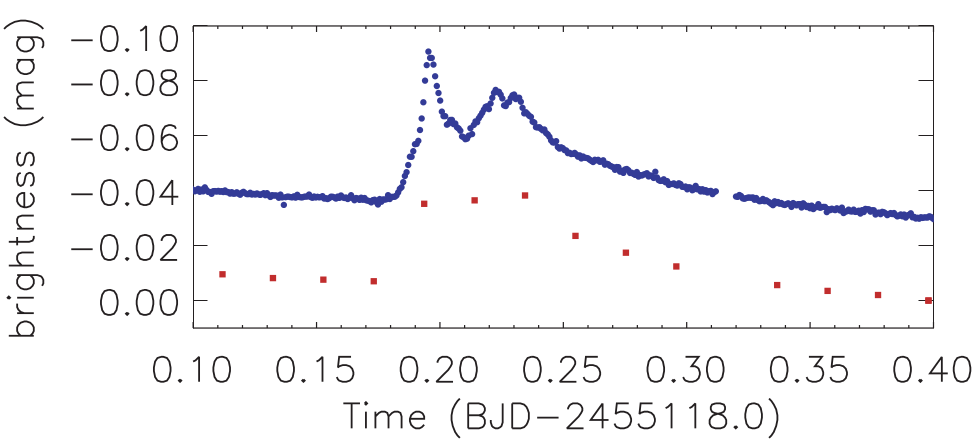
\includegraphics[width=0.80\textwidth]{sc_lc.png}}
\caption{A large-amplitude flare on KIC 12406908. The LC data (red squares) are 
plotted beneath the SC data (blue circles) for comparison. 
The change in brightness is precise, but not accurate – the dimmest LC point was
chosen as the zero-point for the graph, and all SC points are offset for clarity \citep{Murphy2012}.}
\label{fig_sclc}
\end{figure}

\section{Kepler Eclipsing Binary Catalog}

Large samples are useful to determine statistical properties
and for finding rare binaries which may hold physical significance (for example, binaries with very low mass stars,
binaries with stars in short-lived stages of evolution, very eccentric binaries that show large apsidal motion, etc.).
Catalogs of EBs from ground-based surveys suffer from various observational biases such as limited accuracy per
individual measurement, complex window functions (e.g., observations from ground based surveys can only be done
during nights with clear skies and during certain seasons).

The Kepler Eclipsing Binary Catalog lists the stellar parameters from the Kepler Input Catalog (KIC) augmented
by: primary and secondary eclipse depth, eclipse width, separation of eclipse, ephemeris, morphological classification
parameter, and principal parameters determined by geometric analysis of the phased light curve.
The online Catalog also provides the raw and detrended data for ∼30 minutes (long) cadence, and raw ∼1 minutes (short)
cadence data (when available), an analytic approximation via a polynomial chain, and eclipse timing variations. 

The construction of the Catalog consists of the following steps: 
\begin{itemize}[noitemsep]
\item EB signature detection; 
\item data detrending: all intrinsic variability and extrinsic variability are removed by the iterative 
fitting of the photometric baseline; 
\item the determination of the ephemeris: the time-space data are phase-folded and the dispersion minimized; 
\item Determination of ETVs;
\item analytic approximation: every light curve is fit by a polyfit; 
\item morphological classification via Locally Linear Embedding (LLE), a nonlinear dimensionality 
reduction tool is used to estimate the “detachedness” of the system;
\item EB characterization through geometric analysis;
\item diagnostic plot generation for false positive (FP) determination.
\end{itemize}


Only bonafide EBs and systems that clearly exhibit binarity through photometric analysis was accepted for inclusion in this catalog. 
Although best efforts have been taken to provide accurate results, there is caution that not all systems marked in the
Catalog are guaranteed to be EB systems. There remains the possibility that some grazing EB signals may belong to small
planet candidates or are contaminated by non-target EB signals. For now, 2878 objects are identified and analysed from the entire data set
of the primary Kepler mission (Q0-Q17) \citep{kirk2016}. In this work we are dealing with $3^{rd}$ release of this catalog.